\documentclass[conference]{IEEEtran}
\IEEEoverridecommandlockouts
% The preceding line is only needed to identify funding in the first footnote. If that is unneeded, please comment it out.
\usepackage{cite}
\usepackage{amsmath,amssymb,amsfonts}
\usepackage{algorithmic}
\usepackage{algorithm2e}
\usepackage{graphicx}
\usepackage{textcomp}
\usepackage{cleveref}
\usepackage{xcolor}
\usepackage{multirow}
\def\BibTeX{{\rm B\kern-.05em{\sc i\kern-.025em b}\kern-.08em
    T\kern-.1667em\lower.7ex\hbox{E}\kern-.125emX}}
    
\graphicspath{ {./pics/} }
\newcommand{\etal}{\textit{et al}.}

\begin{document}

\title{Supervised-learning Congestion Predictor For Routability-Driven Global Routing\\
}

% \author{\IEEEauthorblockN{1\textsuperscript{st} Given Name Surname}
% \IEEEauthorblockA{\textit{dept. name of organization (of Aff.)} \\
% \textit{name of organization (of Aff.)}\\
% City, Country \\
% email address}
% \and
% \IEEEauthorblockN{2\textsuperscript{nd} Given Name Surname}
% \IEEEauthorblockA{\textit{dept. name of organization (of Aff.)} \\
% \textit{name of organization (of Aff.)}\\
% City, Country \\
% email address}
% \and
% \IEEEauthorblockN{3\textsuperscript{rd} Given Name Surname}
% \IEEEauthorblockA{\textit{dept. name of organization (of Aff.)} \\
% \textit{name of organization (of Aff.)}\\
% City, Country \\
% email address}
% \and
% \IEEEauthorblockN{4\textsuperscript{th} Given Name Surname}
% \IEEEauthorblockA{\textit{dept. name of organization (of Aff.)} \\
% \textit{name of organization (of Aff.)}\\
% City, Country \\
% email address}
% \and
% \IEEEauthorblockN{5\textsuperscript{th} Given Name Surname}
% \IEEEauthorblockA{\textit{dept. name of organization (of Aff.)} \\
% \textit{name of organization (of Aff.)}\\
% City, Country \\
% email address}
% }

\maketitle

\begin{abstract}
    There is on-going development in technology that is pushing the design to an advanced degree of complexity.
    It affects the convergence of physical design, in which routing is one the most critical stages.
    Routability has hit the bottleneck, because congestion estimated by conventional routers does not cope well with modern sophisticated routing parameters, which has an adverse effect on design feasibility.
    Several techniques have recently been developed to predict routability information through a supervised-learning based mechanism.
    However, features extracted by such methods are rather primitive to represent actual physical properties.
    Furthermore, lack of global information led to worse global routing performance.
    In this paper, we propose a supervised-learning regression model which is able to capture accurate global routing behaviours, through which a congestion prediction model is trained to improve the global routing.
    Experimental results show that, in contrast with conventional global-routing-based congestion estimation, our proposed work is at least 9.33$\times$ faster in execution, while maintaining an accurate prediction.
    Moreover, by integrating our model into the router, a better routing topology is achieved, and a superior quality of performance is observed. 
\end{abstract}

\begin{IEEEkeywords}
Back-end design, physical design, placement, routing, routability, supervised data learning
\end{IEEEkeywords}

\section{Introduction}
\label{sec:intro}
\subsection{Motivation}
With the rapid development of technology nodes, design rules become complicated, and numerous of those have imposed upon layouts to secure viable fabrications.
As was discussed in \cite{theimportance}, routability has raised as one of the most important factor to consider during the circuit design workflow, take the minimum spacing rule for example.
Space between two adjacent routes began to depend on the metal width at the 130$nm$ node, and it started to rely on the width of these two adjacent wires at the 65nm node.
This minimum spacing rule becomes more complicated at the 32$nm$ node.
The spacing depends not only on the factors mentioned above but also on their \textit{runlength}, which is the total length of two adjacent wires run parallel.
This phenomenon indicates that one cannot simply sum the widths of all wires in a certain area and assume that this suffices to check whether the routability constraint is satisfied for that said region.
In other words, existing approaches for solving physical design problems such as placement and routing scale poorly or does not scale at all for newer and larger designs.


\subsection{Previous Works}
With the growing design complexity, ``congestion map'' is being used as the metric to deal with routability-driven applications.
It indicates regions where routing will be difficult to achieve.
Attempts to solve this problem are normally taken place in early physical design stages.
Existing approaches can be categorized as follows:
\begin{itemize}
\item \textbf{Static approaches}: Where congestion maps are fixed for placement. The total wirelength of routing regions of the design is calculated using rent's rule in \cite{rentsrule,rentsrulerecursive}, to estimate the corresponding congestion map. However, these algorithms are recursive approach with run-times that scale poorly with the complexity of the design. 
\item \textbf{Probabilistic approaches}: Where net topologies are probabilistically generated based upon placement.  Lou \etal~\cite{first} first proposed a stochastic estimation approach that calculates the demand of all feasible routes that could be taken for each net and assigned them an equal probability. The work in~\cite{modeling} adapted and extended the concept of~\cite{first} such that it restricts the total set of possible routing configurations per net to eliminate impractical or rarely-used ones. Other papers, such as~\cite{SMD, 3step} consider all possible routing configurations in a grid-cell-wise approach to obtain probability distributions.
\item \textbf{Constructive approaches}: Where a global router is used to generate approximated congestion maps by performing a fast routing.  Mainstream global-router-based algorithms~\cite{mixedsizeplacement,ripple,simplr,nctufast,fastroute} are being applied in most routability-driven applications. They are the simplified fully functional global routers with much smaller searching range, higher tolerance and threshold. However, as reported in \cite{fastroute}, the only possible way to accurately predict the routability using global-router-based method is to route the design with the same technique and parameters afterwards. Furthermore, later studies~\cite{study,ispd14,ispd15} show that the global-router-based algorithm did not match the result after the detailed routing, because no local information such as local-pin-number is considered.
\item \textbf{Supervised-learning approaches}: As discussed in \cite{mlinphysicaldesign}, researchers have discovered the beauty of applying various machine learning techniques to solve physical design problems. The work in \cite{drcpredict18} proposed a Design Rule Checking (DRC) violation prediction model which answers yes or no to whether a certain routing region will be having a DRC violation. However, this type of methods have a different programming philosophy from conventional works. As a result, \cite{drcpredict18,drcDAT18} have not embedded the prediction model into design tools, hence the impact on physical design is not observed. On the other hand, \cite{drcingr} takes the DRC prediction into consideration when performing routing. While detailed routing performance is improved, that of global routing is worsen, due to the model limitation that only evaluates local DRC violations.
\end{itemize}


\subsection{Overview of Our Work}
In this paper, we propose a supervised-learning based algorithm to construct accurate routability model which not only considers local information but global resources as well.
The proposed algorithm learns from the placement and global routing instances and extracts highly ranked local attributes as is studied in \cite{parameterstudy}, while taking into account the global routing information.
Experimental results show that our method has a speedup of 9.33$\times$ comparing to pattern-routing based methods, and that of 17.45$\times$ to conventional mainstream global-routing-based approaches.
Moreover, by embedding our prediction model into the design tools, improved performance has been observed not only for global routing, but also routability-driven edge shifting technique proposed in \cite{fastroute}.
Detailed discussion is presented in Section \ref{sec:result}. 

Our key contributions are as follows:
\begin{itemize}
\item We present a supervised-learning congestion prediction algorithm to efficiently generate routability model.
\item Define and extract effective features at post-placement stage.
\item A probabilistic algorithm is developed and embedded into our algorithm as a feature for model training.
\item The proposed model has been embedded into the global router to optimise routing topology.
\end{itemize}

The rest of the paper is organised as follows.
\Cref{sec:prelim} explains the problem formulation and terminology related to routability optimisation.
In \Cref{sec:methodology}, the proposed framework is presented.
The results are discussed in \Cref{sec:result}. Finally, conclusion is presented in \Cref{sec:conlu}.

\section{Preliminaries}
\label{sec:prelim}

\subsection{Grid Model}
\label{subsec:grid model}

\begin{figure}[tb!]
    \centering
    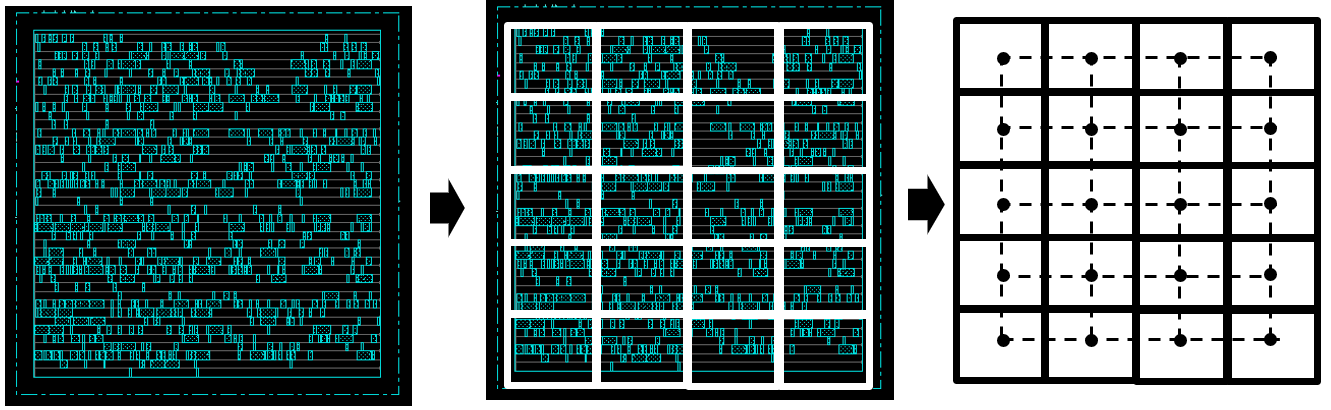
\includegraphics[width=3in]{grid_model}
	\caption{The design is divided into rectangular tiles (solid lines). The dark
		circles and dashed lines represent the vertices and the edges of the grid graph, respectively.}
	\label{fig:grid_model}
\end{figure}

Global routing is performed on a grid which is the logical graph representation of the physical chip. The grid graph \emph{G} is tile-based, which means that the entire chip is partitioned into multiple sub-regions, as illustrated in Fig.~\ref{fig:grid_model}. Each sub-region is referred to as a grid cell, or a global routing cell. The cells are further subdivided with vertical and horizontal gridlines, i.e., along which routes are determined and wires can be created. Each vertex in \emph{G} represents a corresponding tile, and each edge in \emph{G} between vertices corresponds to the shared boundary of two tiles.

\subsection{Routing Metrics}
\subsubsection{Routing Capacity}
The graph \emph{G} used for global routing needs to capture the capacities of the routing regions. The capacity of an edge \emph{e} $\in$ \emph{G} between two vertices \emph{u} and \emph{v} is defined as the maximum number of available routing tracks between the routing regions of \emph{u} and \emph{v}. 

High-precision capacity metric can be complex and possible in practice, such track-based capacity can be extended to consider specific routing elements such as blockages, vias, and fixed pins. Such elements have different penalties to their respective edge capacity. For example, blockages may consume the capacity of an entire edge. 

\subsubsection{Overflow}
If the total usage of an edge $e$ is larger than its capacity, then the tile containing that edge is considered to be congested, and the amount of overhead is referred to as {\it overflow}, $of(e)=\text{usage}(e)-\text{capacity}(e)$. Detailed routing would not be able to route all nets assigned to congested areas due to lack of routing resources. However, there is generally a degree of tolerance as a detailed router may be able to spread the routes from the congested tiles to adjacent less-congested ones, if those are available. Not only do global routing paths contribute to the usage of edge, other factors, such as local pins, could cause an overflow as well by decreasing edge capacity.
% \subsubsection{Wirelength}
% The minimization of wirelength is another important metric for global routing. Decreased wirelength implies smaller power consumption and delays, which are two key factors for  performance-driven optimization. Inherently, congestion minimization conflicts with wirelength minimization, because detours may be introduced to avoid congested regions and that leads to longer wirelength. Therefore, the trade-off between these features has to be carefully tuned based on the requirements of circuit design. 

\subsection{Routability Problem Formulation}
The key objective is to maximize the routability of a design, which is used as a metric to predict the overall quality of routing generated for a design subjected to nets and other design constraints.
Thus the routing problem can be formulated as follows:
\begin{subequations}
\begin{align*}
    \max  \       & f(X), \\
    \text{s.t.}~~ & d(X) \leq 0, \\
                  & n(X) \leq 0,
\end{align*}
\end{subequations}
where f(X) is the measure of quality (routability), and $n(X)$ denotes network constraints and $d(x)$ denotes a set of other design constraints.  Network constraints indicate that the topology of the network must satisfy certain requirements, e.g., pins of each net all have to be  connected without loops. On the other hand, design constraints are to ensure that the implementation of the network topology meets certain requirements, e.g., the routing direction follows a layer's specifications. Our work fits within the routability optimization problem.

\subsection{Supervised Data Learning Technique}
Data learning is a powerful technique which can drive knowledge from large amounts of data to predict and generalize unseen data patterns. In the research field of physical design algorithms, supervised learning is widely used.

As illustrated in Fig.~\ref{fig:ml_flow}, given certain features as input, the training process builds a set of models which are subsequently evaluated. One way of testing the quality of models is to feed the same input features as those fed during training to see how closely the predicted values match the the original target output. After such an evaluation, acceptable models are selected for making the predictions in two sets of machine learning applications. 
\begin{figure}[tb!]
    \centering
    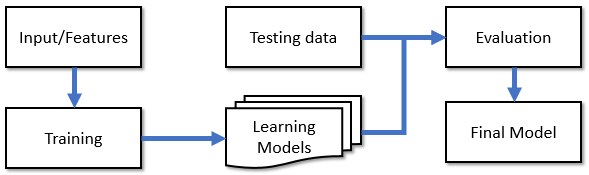
\includegraphics[width=.68\linewidth]{ML_flow}
    \caption{Supervised learning flow.}
    \label{fig:ml_flow}
\end{figure}
There are two types of applications: Regression and classification \cite{MLtypes}.

\section{Proposed Methodology}
\label{sec:methodology}
Our machine learning algorithm is required to predict the global routing pattern of a design. Thus, it needs to be trained to create an accurate predictive model. For the purpose of training, certain features need to be extracted from designs that have already undergone global routing. Along with these features, post-routing congestion information for each edge needs to be extracted. Two matrices, one containing these features and another populated with the congestion information act as input and output values required to train the machine learning model. 

We use NTHU-Route 2.0 \cite{NTHU} as the platform to implement our routability model. Since the congestion in this router is calculated using an edge-based perspective, all the features of the design are observed using a similar approach. 

\subsection{Routing Feature Extraction}
\begin{itemize}
\item \textbf{First-degree pins}. First degree pins are pins closest to an edge and are deemed to have a significant impact on the probability of the routing wire to cross-over the chosen edge, thus altering its congestion value. \Cref{fig:fdpin} depicts a visual representation of this feature. This feature provides a metric for the proximity or vicinity of pins with respect to an edge. To route a first-degree pin, at least one of the four edges surrounding that pin will be crossed by the wire.

\begin{figure}[tb!]
    \centering
    \subfloat[]{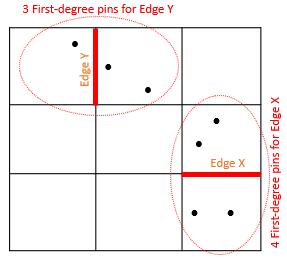
\includegraphics[width=.48\linewidth]{fdpin}  \label{fig:fdpin}}
    \subfloat[]{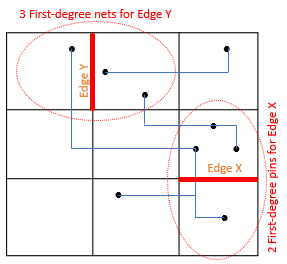
\includegraphics[width=.48\linewidth]{fdnet}  \label{fig:fdnet}}
    \caption{Examples of (a) first degree pins; (b) first degree nets.}
\end{figure}

\item \textbf{First-degree nets}. A tile can contain various pins which belong to different nets. Different pins in a tile can be a part of the same net or part of different nets. The first-degree nets of an edge are those nets that passes either of the two tiles that the said edge is a part of, \Cref{fig:fdnet}  gives an example of this feature. 

\item \textbf{Pin density}. This ``density'' feature gives information regarding the number of pins per unit area. Pin density for a chosen edge is given by the number of first-degree pins of that edge divided by two tiles that this edge is a part of. Pin density helps to give information of how congested the pins are within a tile which directly translates to a higher probability for the tile's corresponding edges to be used for routing. A higher pin density means that the edges of this tile can mostly be used to route pins within that tile. This deems the edges unroutable for wire connecting other tiles and thus a detour must be made. 

\item \textbf{RSMT-aware two-pin path distribution}. This ``distribution'' feature represents in the evaluation of the most appropriate path for global routing based on a probabilistic model. The router initially creates multi-pin net RSMT structures using the FLUTE \cite{FLUTE} and then fragments each structure into two-pin pairs. Given the location of two pins, various paths are constructed from one to the other, as is shown in \Cref{fig:2pinusage}. Subsequently, the ‘total availability’ for each path is calculated. This total availability depends on the maximum capacity of each edge lying in the chosen path. Please note that the user has the freedom of choosing what paths to consider, such as L-shape, Z-shape, and monotonic. More shapes can provide enhanced accuracy, but comes with a computational time penalty.

\begin{figure}[tbh!]
    \centering
    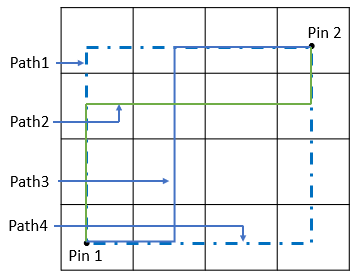
\includegraphics[width=1.5in]{2pinusage}
    \caption{Four possible paths for a two-pin net.}
    \label{fig:2pinusage}
\end{figure}

If $n$ edges constitute a path $i$, and let $M(e)$ be the maximum capacity for an edge $e$, then the total availability $A(i)$ for the path $i$ is $A(i)=\sum_{e=0}^{n}M(e)$. Note that for any edge $e$ in the path $i$, if $M(e)=0$, then the entire path is eliminated from candidacy. Following the computation of the total availability of each of the potential paths, the probability of each path is calculated. This calculation is done by obtaining the sum of the total availability of all potential paths between the two pins as shown in \Cref{fig:2pinusage}.
If there are k paths, the probability of path $p(i)=\frac{A(i)}{\sum^{k}A}$

Each edge $j$ in path $i$ is assigned a probability $p(i)$ which reflects its likelihood for being used in global routing. Since an edge can belong to more than one potential path, the usage assigned to each edge is a sum of all the path probabilities of which this chosen edge is a part of. Thus, we acquire probabilistic information for each edge to be used in global routing. In an edge-based analyses, this feature provides us valuable information for the routing probability of an edge from a standalone perspective.

\begin{figure}[tb!]
    \centerline{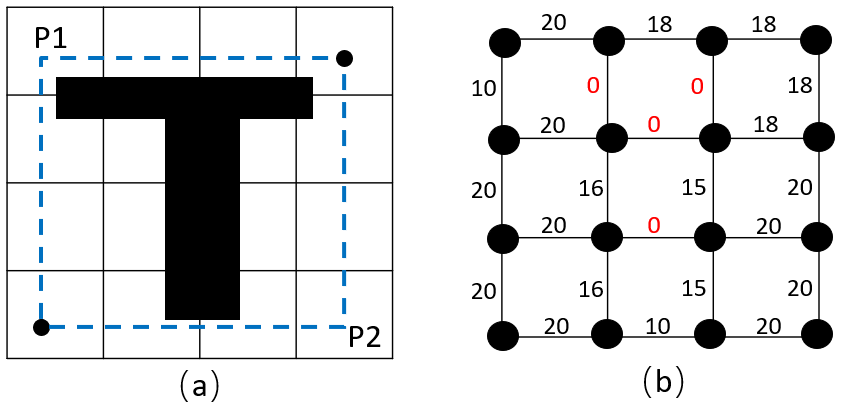
\includegraphics[width=2.6in]{2pinexample}}
    \caption{(a) A design grid with blockage and two possible paths; (b) Corresponding routing graph and related edge capacity.}
    \label{fig:2pinexample}
\end{figure}
An simple example is shown in \Cref{fig:2pinexample}, there are two possible paths, P1 and P2, for routing the pin-pair, where two pins are located at the lower left and upper right corners. From the routing graph, we obtain $A(P1)=106$ and $A(P2)=108$. So the probability of choosing path P1 is $p(P1)=106/(106+108)=0.49$, therefore $p(P2)=0.51$. The final usage assigned for edges passed by these two paths will then be increased by either 0.49 or 0.51, accordingly.
\end{itemize}

\subsection{Routability-Driven Edge Shifting}
We use our routability information to guide the edge shifting technique in FLUTE\cite{fastroute}. The congestion map heavily affects the structure of Steiner tree, hence the actual routing. Therefore, the quality of the congestion map directly affects that of the tree topology.

To perform shifting is to move Steiner points. The edge that connects at least one Steiner point is selected. The moving direction for the Steiner point is perpendicular to the edge, and the allowed range for moving the said Steiner point is determined by other paths that connect to the two endpoints of the shifting edge, whichever is shorter. As is demonstrated in \Cref{fig:edgeshifting}, the edge-to-shift is horizontal, therefore, the Steiner point is moving in a vertical direction, and the range of moving is determined by the shortest path which previously connected the left endpoint of the shifting edge. 
\begin{figure}[htbp]
    \centerline{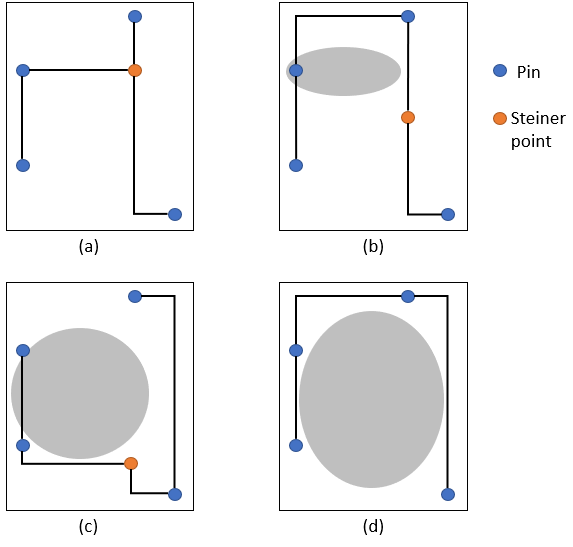
\includegraphics[height=1.8in, width=2.7in]{edgeshifting}}
    \caption{(a) The initial Steiner tree (b) Allowed moving area for Steiner point (c)(d) Modified tree structures based on different congestion map.}
    \label{fig:edgeshifting}
\end{figure}

\subsection{Prediction Model Embedded Routability Optimization}
After the features are extracted, we use MARS \cite{MARS} to predict routability. The reasons of selecting MARS are as follows: 1) Interactions between independent parameters can be captured. 2) Non-linearity can be modeled. 3) Tuning is easy, and in most cases, not needed. 

We pick a median-size design and extract corresponding features.
After a model is trained, we select as testing data three other designs with respective small median and large size.
A model is deemed acceptable if its max-min congestion range of prediction is within 15\% comparing with that of actual.
Then, the congestion model is integrated into the global router, as is shown in \Cref{alg:route}.
After necessary initialization such as reading design and creating routing graph, initial Steiner trees are constructed for each net by using FLUTE \cite{FLUTE} (line \ref*{alg:ln:flute}).
The congestion map is generated by our model and assigned to each edge of the graph (line \ref*{alg:ln:cong}).
Shifting lines for each Steiner point is determined as the first step of edge shifting,
along which the Steiner point moves to find the least congested spot to optimize the tree structure (line \ref*{alg:ln:es}).
After the Steiner tree is adjusted and the routing topology is conducted, the routing follows (line \ref*{alg:ln:routing}).
The router starts from each optimized tree of nets, and choose the best path candidate based on the congestion map, and finally construct a fully routed design layout.
Once the routing is finished, the actual congestion is produced by real routing path
. Congestion map which previously read from model is then removed (line \ref*{alg:ln:rmcong}), to avoid interference between two kinds of information, predicted and actual, in the final stage.
A Rip-up \& Reroute is performed at last while judging the threshold at each iteration (line \ref*{alg:ln:rrr}).


\begin{algorithm}
    \caption{Routability Model Guided Routing}
    \label{alg:route}
    \begin{algorithmic}[1]
        \Require Placed netlist.
        \State \texttt{Init()};
        \While{net $\gets$ nets.\texttt{read}()}
            \State \texttt{FLUTE}(net); \label{alg:ln:flute}
            \State congestion $\gets$ \texttt{inputGuide}(model); \label{alg:ln:cong}
            \State \texttt{edgeShifting}(net, congestion); \label{alg:ln:es}
            \State \texttt{routing}(net, congestion); \label{alg:ln:routing}
            \State \texttt{removeGuide}(congestion); \label{alg:ln:rmcong}
            \While{FALSE == \texttt{metThreshold}()}
                \State \texttt{ripUpReroute}(); \label{alg:ln:rrr}
            \EndWhile
        \EndWhile
    \end{algorithmic}
\end{algorithm}

% \iffalse
% \begin{algorithm}
% \SetAlgoLined
% \KwResult{Global Routing Instance}
%  initialisation()\;
%  \While{net = nets.read()}{
%     FLUTE(net)\;
%     congestion = inputGuide(model)\;
%     edgeShifting(net, congestion)\;
%     routing(net, congestion)\;
%     removeGuide(congestion)\;
    
%     \While{!metThreshold()}{
%         ripUpReroute()\;
%         }
  
%  }
%  \caption{routability model guided routing}
% \end{algorithm}
% \fi

\section{Experimental Result}
Data set is obtained from ISPD'08 benchmarks since NTHU-Route 2.0 only accepts this format. ten designs are chosen for experiments, four other designs cannot be routed using NTHU-Route 2.0, therefore are not considered. The experiment was run on linux workstation with X-core X.XXGHz CPU and XXGB memory. The 2-pin usage attribute is set to consider L-shape only, which is meant to illustrate the importance of capturing hidden parameter interactions when calculating routability. Because other attributes are also extracted along with L-shapes when training models and predicting congestion, the difference between the routing performance with and without our methods can be considered the impact of our work.

\subsection{Runtime comparison}
The NTHU-Route 2.0 uses bounding-box routing technique to generate the initial congestion map on which the routability-driven edge shifting is performed. However, for the purpose of routing and other applications such as routability-driven placement, the final congestion map produced by NTHU is generated after the edge shifting and L-shape pattern routing. The runtime comparison is shown in Table \ref{tab:runtime}. The runtime of the bounding box routing algorithm, full estimation and extraction are all directly proportional to the design size. However, extraction is much simpler in contrast to the routing algorithms. We achieved speedups of 9.33X and 17.45X, comparing with bounding box routing and NTHU-Route's estimation method.
\begin{table*}[htbp]
\caption{congestion estimation runtime comparison}
\begin{center}
\begin{tabular}{|c|c|c|c|c|c|}
\hline
\multirow{2}{*}{Benchmark} & \multicolumn{2}{l|}{NTHU-Route 2.0 \cite{NTHU}} & \multicolumn{3}{l|}{Proposed Work}        \\ \cline{2-6} 
                           & Bbox Route   & Full Estimation  & Attribute Extraction & Prediction & Total \\ \hline
adaptec1                   & 2.02         & 6.49             & 0.42                 & 0.11       & 0.53  \\ \hline
adaptec2                   & 2.74         & 5.81             & 0.35                 & 0.13       & 0.48  \\ \hline
adaptec3                   & 11.25        & 20.36            & 0.63                 & 0.5        & 1.13  \\ \hline
adaptec4                   & 12.16        & 20.62            & 0.58                 & 0.51       & 1.09  \\ \hline
adaptec5                   & 9.52         & 19.08            & 0.89                 & 0.22       & 1.11  \\ \hline
bigblue1                   & 1.60         & 4.93             & 0.31                 & 0.05       & 0.36  \\ \hline
newblue1                   & 2.29         & 4.74             & 0.39                 & 0.2        & 0.59  \\ \hline
newblue2                   & 5.22         & 9.85             & 0.47                 & 0.20       & 0.67  \\ \hline
newblue5                   & 19.71        & 34.5             & 1.18                 & 0.35       & 1.53  \\ \hline
newblue6                   & 13.90        & 24.06            & 0.96                 & 0.17       & 1.13  \\ \hline
Average                    & 9.33X        & 17.45X           & n/a                  & n/a        & 1.00X \\ \hline
\end{tabular}
\label{tab:runtime}
\end{center}
\end{table*}

\subsection{Impact on routability-driven edge shifting}
In order to evaluate the quality of Steiner Tree structure, after all nets of a design has done routability-driven edge shifting, we perform L-shape routing on the optimized topology. The bounding box routing estimation only considers the boundaries of 2-pin boxes, which is the equivalent of performing L-shape routing twice without taken into account other factors. As is mentioned in \cite{fastroute}, only the same technique of routing is being applied for congestion estimation, can we obtain an relatively accurate congestion map for that router. Therefore, L-shape routing is chosen for routing.

We first take adaptec3 as an special case and exclude it, since its total overflow is too abnormal while other two factors stayed in range. This might happen due to the uncontrollable model behaviour which we have not yet fully investigated. As is shown in Table \ref{tab:treequality}, maximum overflow (Max\_OF) has decreased 18\% and total overflow (Total\_OF) has dropped 9\%. Please note that the wirelength (WL) has only changed less than 1\%, which means almost no detour is made, the Steiner Tree topology optimized using our congestion map did avoid congested regions before routing is carried out.



\begin{table*}[htbp]
\caption{Result of Steiner Tree quality after edge shifting}
\begin{center}
\begin{tabular}{|c|c|c|c|c|c|c|}
\hline
\multirow{2}{*}{Benchmark} & \multicolumn{3}{l|}{Bounding Box Routing}     & \multicolumn{3}{l|}{Our Work}  \\ \cline{2-7} 
                           & WL       & Max\_OF & Total\_OF      & WL       & Max\_OF & Total\_OF \\ \hline
adaptec1                   & 3391427  & 112     & 245459 (+20\%) & 3391361  & 77      & 203315    \\ \hline
adaptec2                   & 3207461  & 93      & 152268 (+15\%) & 3207459  & 92      & 132709    \\ \hline
adaptec3                   & 9346466  & 80      & 593070 (-90\%) & 9346462  & 75      & 4947842   \\ \hline
adaptec4                   & 8891886  & 75      & 220259 (+63\%) & 8891797  & 63      & 134954    \\ \hline
adaptec5                   & 9505500  & 132     & 603652 (+8\%)  & 9805443  & 116     & 559175    \\ \hline
bigblue1                   & 3433454  & 76      & 218667 (+1\%)  & 3433406  & 66      & 217006    \\ \hline
newblue1                   & 2325703  & 52      & 52556 (-1\%)   & 2325657  & 43      & 52821     \\ \hline
newblue2                   & 4604357  & 89      & 77374 (+42\%)  & 4604356  & 67      & 54487     \\ \hline
newblue5                   & 14230198 & 155     & 627669 (+13\%) & 14230009 & 123     & 556639    \\ \hline
newblue6                   & 9755863  & 103     & 475561 (-12\%) & 9755823  & 106     & 544858    \\ \hline
Average (ex. adaptec3)     & 0.99     & 1.18    & 1.09           & 1        & 1       & 1         \\ \hline
\end{tabular}
\label{tab:treequality}
\end{center}
\end{table*}

\subsection{Global Routing Performance}
The executable compiled from NTHU-Route source code could not successfully run through the post-processing for some of the designs. Therefore, we are only comparing the output in the first phase. The overflow threshold is set to be 200, which means the router will proceed to post-processing when overflow goes below 200 during iterations. The post-processing is a process to erase the history cost of all edges from the router's record, so that the edges previously visited but not heavily occupied can be freed as valid candidates again. 

We can observe from the Table \ref{tab:gr} that by applying our congestion map, the Total\_OF of all designs are smaller than corresponding ones, summed up in a total of 10\% improvment. Lower Total\_OF represents a higher chance of being successfully routed. Moreover, it would lighten the task of the post-processing. Also worth noticing, the Total\_OF of adaptec2, adaptec3, newblue2 all have a large gap between using original and our congestion map. by modifying the threshold value based upon these experimental data, we can reduce the number of iterations. Other factors are tied, which means it is feasible that we can replace the original pattern-route based congestion estimation by the output of our data-learning based congestion prediction model.


\begin{table*}[htbp]
\caption{Result of Global Routing Performance}
\begin{center}
\begin{tabular}{|c|c|c|c|c|c|c|c|c|}
\hline
\multirow{2}{*}{Benchmark} & \multicolumn{4}{l|}{NTHU-Route 2.0}          & \multicolumn{4}{l|}{NTHU-Route 2.0 with Our Work} \\ \cline{2-9} 
                           & \#iteration & Max\_OF & Total\_OF & WL       & \#iteration   & Max\_OF  & Total\_OF  & WL        \\ \hline
adaptec1                   & 11          & 2       & 170       & 3595770  & 11            & 2        & 166        & 3593832   \\ \hline
adaptec2                   & 12          & 2       & 197       & 3307228  & 12            & 2        & 175        & 3306489   \\ \hline
adaptec3                   & 8           & 2       & 177       & 9471843  & 8             & 2        & 128        & 9670341   \\ \hline
adaptec4                   & 4           & 4       & 116       & 8970266  & 4             & 4        & 115        & 8967345   \\ \hline
adaptec5                   & 14          & 2       & 173       & 10307879 & 14            & 2        & 143        & 10306712  \\ \hline
bigblue1                   & 16          & 2       & 143       & 3719329  & 15            & 2        & 198        & 3716884   \\ \hline
newblue1                   & 23          & 2       & 191       & 2398649  & 23            & 2        & 184        & 2402800   \\ \hline
newblue2                   & 3           & 4       & 197       & 4643206  & 4             & 4        & 112        & 4642987   \\ \hline
newblue5                   & 16          & 2       & 182       & 14701827 & 16            & 2        & 174        & 14701360  \\ \hline
newblue6                   & 17          & 2       & 172       & 10270966 & 17            & 2        & 172        & 10270966  \\ \hline
Average                    & 1.00        & 1.00    & 1.10      & $\approx$1 & 1           & 1        & 1            & 1  \\ \hline
\end{tabular}
\label{tab:gr}
\end{center}
\end{table*}
\section{Conclusion}
\label{sec:conlu}

We addressed the global routing optimisation problem using supervised-learning based algorithms.
We showed that recent approaches that extract design features are not sufficient for achieving desirable global routing performance.
We proposed a regression algorithm that uses advanced features for model training and congestion prediction, which is at least 9.33 times faster than conventional methods.
We then embedded our model into Steiner tree edge shifting and observed that final  routing topology is improved in terms of having fewer \text{Max\_OF} and \text{Total\_OF}.
We also implemented the model in a global router to evaluate the effectiveness of our proposed algorithm.
Our experiments show that, without negatively impacting timing convergence, we are able to improve the routing performance by reducing 10\% of total overflow and a case-wise 4.8\% runtime speedup.
Our future works include (1) improving the model accuracy, (2) combining  detailed routing features to optimise detailed routing, and (3) applying our methodology to emerging technology nodes.


\bibliographystyle{IEEEtran}
\bibliography{./ref/Top,./ref/IEEEabrv}

\end{document}
